\documentclass[conference]{IEEEtran}
\IEEEoverridecommandlockouts
% The preceding line is only needed to identify funding in the first footnote. If that is unneeded, please comment it out.
\usepackage{cite}
\usepackage{amsmath,amssymb,amsfonts}
\usepackage{algorithmic}
\usepackage{graphicx}
\usepackage{textcomp}
\usepackage{xcolor}
\usepackage{tikz}
\usepackage{booktabs}
\usetikzlibrary{shapes.geometric, arrows, arrows.meta, positioning, fit, calc, backgrounds}

\def\BibTeX{{\rm B\kern-.05em{\sc i\kern-.025em b}\kern-.08em
    T\kern-.1667em\lower.7ex\hbox{E}\kern-.125emX}}

\begin{document}

\title{Efficient Vision-Language-Action Models via Hybrid Diffusion Heads\\
}

\author{\IEEEauthorblockN{1\textsuperscript{st} Given Name Surname}
\IEEEauthorblockA{\textit{dept. name of organization (of Aff.)} \\
\textit{name of organization (of Aff.)}\\
City, Country \\
email address or ORCID}
}

\maketitle

\begin{abstract}
Vision-Language-Action (VLA) models map images, language and robot state to actions, but adapting a pre-trained VLA to a specific task usually means fine-tuning hundreds of millions of parameters. We study a cheaper alternative: the VLA is kept completely frozen and a small generative head is trained on top of it. Our \emph{hybrid diffusion} head is a conditional flow-matching model that predicts a \emph{residual} action chunk. It is conditioned on (i) a pooled semantic feature from the frozen SmolVLA backbone and (ii) the action chunk that the frozen SmolVLA policy itself proposes for the same observation; the executed action is the base action plus the sampled residual. Because the backbone is frozen, its outputs are computed once per demonstration frame and cached, so the 8.5\,M-parameter head trains in about two minutes on one GPU. In a first experiment on one LIBERO-10 task (task 3), the residual policy succeeds in 48 of 50 episodes against 43 of 50 for the frozen base policy on the same initial states. This difference is encouraging but not statistically significant at this sample size (exact McNemar $p=0.125$); evaluation on the remaining LIBERO-10 tasks is in progress.
\end{abstract}

\begin{IEEEkeywords}
Vision-Language-Action, Diffusion Models, Flow Matching, Residual Policy Learning, Imitation Learning
\end{IEEEkeywords}

\section{Introduction}
End-to-end robotic manipulation relies on mapping high-dimensional observations (camera images, robot proprioception) and a natural-language instruction to continuous action sequences. Vision-Language-Action (VLA) models such as RT-2~\cite{rt2}, OpenVLA~\cite{openvla}, $\pi_0$~\cite{pi0} and SmolVLA~\cite{smolvla} show that pre-trained Vision-Language Models (VLMs) can be turned into capable robot policies.

A pre-trained VLA is rarely perfect on a given task. On LIBERO-10~\cite{libero}, the public SmolVLA checkpoint used in this work succeeds on roughly 41\% of episodes on average, with per-task rates between 0\% and 90\% (Table~\ref{tab:results}). The standard remedy, fine-tuning the VLA, is expensive and risks degrading what the model already does well. Diffusion policies~\cite{diffusionpolicy} are a strong alternative for imitation learning, but training one from scratch discards the semantic grounding of the VLA.

We ask whether a small generative head attached to a \emph{frozen} VLA can improve it. Our \emph{hybrid diffusion} approach keeps every SmolVLA weight fixed and trains a lightweight conditional flow-matching head that outputs a correction to the base policy's action chunk. The design rests on three points, each of which we found necessary in practice:
\begin{itemize}
    \item \textbf{The residual is conditioned on the base action it corrects.} The base policy is itself a stochastic sampler, so a residual is only well defined relative to one particular base sample. The head therefore receives that sample as an input.
    \item \textbf{Training and rollout use the same base sampler and the same observation pipeline.} The residual target is computed against the action chunk the base policy would actually execute (same number of integration steps, same rendered observation), not against a cheaper approximation.
    \item \textbf{Frozen-backbone outputs are cached.} The semantic feature and the base action chunks are computed once per demonstration frame, which reduces head training to a few minutes.
\end{itemize}

\section{Related Work}
\subsection{Vision-Language-Action Models}
VLA models co-train or fine-tune large vision-language models on robot demonstrations. RT-2~\cite{rt2} and OpenVLA~\cite{openvla} emit discretised action tokens, whereas $\pi_0$~\cite{pi0} and SmolVLA~\cite{smolvla} attach a flow-matching action expert that generates continuous action chunks while attending to the VLM's internal representations. SmolVLA, used here, is built on the SmolVLM2-500M backbone.

\subsection{Diffusion and Flow-Matching Policies}
Diffusion Policy~\cite{diffusionpolicy} formulates control as conditional denoising of an action trajectory~\cite{ddpm}. Flow matching~\cite{flowmatching} trains a velocity field that transports noise to data along straight paths and is sampled with a few Euler steps. Such policies represent multi-modal action distributions well, but typically rely on visual encoders without language grounding.

\subsection{Residual Policies}
Residual policy learning~\cite{residualpolicy,residualrl} keeps a base controller fixed and learns an additive correction. It has mostly been studied with reinforcement learning on top of a deterministic controller. Our setting differs in two respects: the correction is learned purely from demonstrations, and the base policy is stochastic, which motivates conditioning the residual model on the sampled base action.

\section{Method}

Fig.~\ref{fig:architecture} gives an overview. At every control step the frozen SmolVLA processes the observation once. That single pass yields a semantic feature and a base action chunk; the trainable head turns these into a residual chunk; and the sum of the two is executed.

\begin{figure*}[t]
\centering
\resizebox{\textwidth}{!}{%
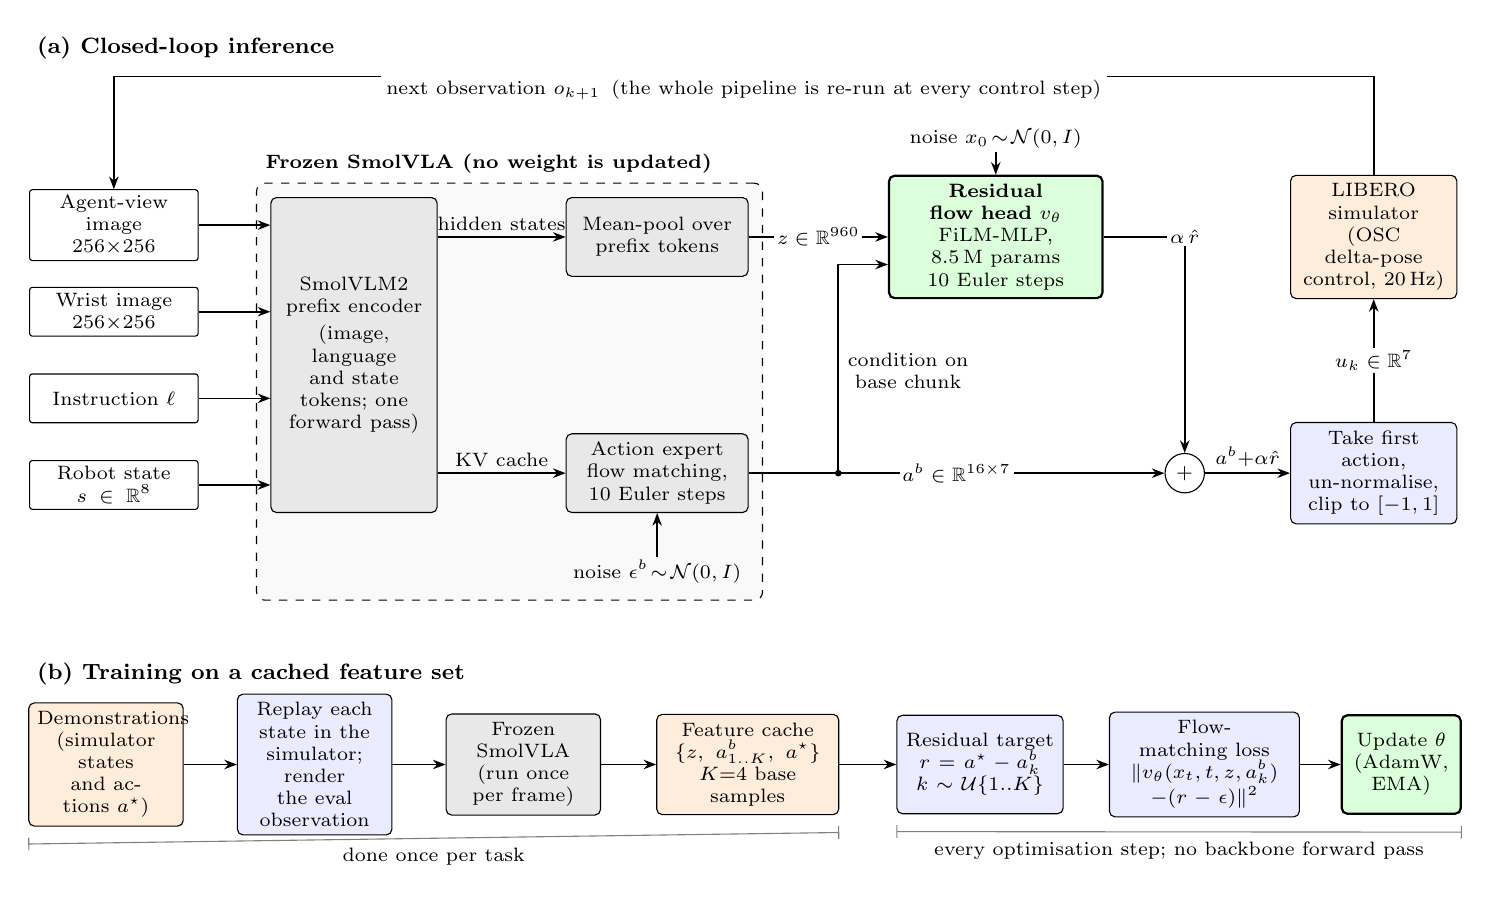
\begin{tikzpicture}[
    font=\scriptsize, >={Stealth[length=1.6mm]},
    inp/.style={draw, rounded corners=1pt, fill=white, text width=2.0cm, align=center, minimum height=0.62cm, inner sep=2pt},
    frz/.style={draw, rounded corners=2pt, fill=gray!18, align=center, inner sep=3pt},
    trn/.style={draw, rounded corners=2pt, fill=green!14, align=center, inner sep=3pt, thick},
    op/.style={draw, rounded corners=2pt, fill=blue!8, align=center, inner sep=3pt},
    dat/.style={draw, rounded corners=2pt, fill=orange!14, align=center, inner sep=3pt},
    nz/.style={align=center, inner sep=1pt},
    arr/.style={->, semithick},
    lbl/.style={midway, fill=white, inner sep=1pt}
]
% ---------------- (a) inference ----------------
\node[inp] (i1) at (0, 1.65) {Agent-view image\\$256{\times}256$};
\node[inp] (i2) at (0, 0.55) {Wrist image\\$256{\times}256$};
\node[inp] (i3) at (0,-0.55) {Instruction $\ell$};
\node[inp] (i4) at (0,-1.65) {Robot state $s\in\mathbb{R}^{8}$};

\node[frz, text width=1.9cm, minimum height=4.0cm] (enc) at (3.05,0) {SmolVLM2\\prefix encoder\\[2pt](image, language and state tokens; one forward pass)};
\node[frz, text width=2.1cm, minimum height=1.0cm] (pool) at (6.9, 1.5) {Mean-pool over prefix tokens};
\node[frz, text width=2.1cm, minimum height=1.0cm] (exp) at (6.9,-1.5) {Action expert\\flow matching,\\10 Euler steps};
\node[nz] (nb) at (6.9,-2.75) {noise $\epsilon^{b}\!\sim\!\mathcal{N}(0,I)$};

\begin{scope}[on background layer]
\node[draw, dashed, rounded corners=3pt, fill=gray!5, fit=(enc)(pool)(exp)(nb), inner sep=5pt] (fbox) {};
\end{scope}
\node[anchor=south west, font=\scriptsize\bfseries] at (fbox.north west) {Frozen SmolVLA (no weight is updated)};

\node[trn, text width=2.5cm, minimum height=1.25cm] (head) at (11.2, 1.5) {\textbf{Residual flow head} $v_\theta$\\FiLM-MLP, 8.5\,M params\\10 Euler steps};
\node[nz] (nh) at (11.2, 2.75) {noise $x_{0}\!\sim\!\mathcal{N}(0,I)$};
\node[draw, circle, inner sep=1pt, minimum size=0.5cm, fill=white] (sum) at (13.6,-1.5) {$+$};
\node[op, text width=1.9cm, minimum height=1.0cm] (post) at (16.0,-1.5) {Take first action,\\un-normalise,\\clip to $[-1,1]$};
\node[dat, text width=1.9cm, minimum height=1.0cm] (env) at (16.0, 1.5) {LIBERO simulator\\(OSC delta-pose\\control, 20\,Hz)};

\foreach \n/\y in {i1/1.65, i2/0.55, i3/-0.55, i4/-1.65} \draw[arr] (\n.east) -- (enc.west |- 0,\y);
\draw[arr] (enc.east |- pool) -- (pool.west) node[lbl, above=1pt, fill=none] {hidden states};
\draw[arr] (enc.east |- exp) -- (exp.west) node[lbl, above=1pt, fill=none] {KV cache};
\draw[arr] (nb) -- (exp);
\draw[arr] (nh) -- (head);
\draw[arr] (pool.east) -- (head.west) node[pos=0.55, lbl] {$z\in\mathbb{R}^{960}$};
\coordinate (tap) at (9.2,-1.5);
\draw[arr] (exp.east) -- (sum.west) node[pos=0.74, lbl] {$a^{b}\in\mathbb{R}^{16\times 7}$};
\fill (tap) circle (1.2pt);
\draw[arr] (tap) |- ($(head.west)+(0,-0.35)$);
\node[nz, anchor=west] at (9.28,-0.2) {condition on\\base chunk};
\draw[arr] (head.east) -| (sum.north) node[pos=0.75, lbl] {$\alpha\,\hat r$};
\draw[arr] (sum.east) -- (post.west) node[lbl, above=1pt, fill=none] {$a^{b}{+}\alpha\hat r$};
\draw[arr] (post.north) -- (env.south) node[lbl] {$u_k\in\mathbb{R}^{7}$};
\draw[arr] (env.north) -- ++(0,1.25) -| (i1.north);
\node[fill=white, inner sep=2pt] at (8.0,3.37) {next observation $o_{k+1}$ \,(the whole pipeline is re-run at every control step)};
\node[anchor=west, font=\footnotesize\bfseries] at (-1.1,3.9) {(a) Closed-loop inference};

% ---------------- (b) training ----------------
\begin{scope}[yshift=-5.2cm]
\node[anchor=west, font=\footnotesize\bfseries] at (-1.1,1.15) {(b) Training on a cached feature set};
\node[dat, text width=1.75cm, minimum height=1.25cm] (demo) at (-0.1,0) {Demonstrations\\(simulator states\\and actions $a^{\star}$)};
\node[op,  text width=1.75cm, minimum height=1.25cm] (replay) at (2.55,0) {Replay each state in the simulator; render the eval observation};
\node[frz, text width=1.75cm, minimum height=1.25cm] (fz) at (5.2,0) {Frozen SmolVLA\\(run once\\per frame)};
\node[dat, text width=2.1cm, minimum height=1.25cm] (cache) at (8.05,0) {Feature cache\\$\{z,\;a^{b}_{1..K},\;a^{\star}\}$\\$K{=}4$ base samples};
\node[op,  text width=1.9cm, minimum height=1.25cm] (res) at (11.0,0) {Residual target\\$r=a^{\star}-a^{b}_{k}$\\$k\sim\mathcal{U}\{1..K\}$};
\node[op,  text width=2.2cm, minimum height=1.25cm] (loss) at (13.85,0) {Flow-matching loss\\$\lVert v_\theta(x_t,t,z,a^{b}_{k})$\\$-(r-\epsilon)\rVert^{2}$};
\node[trn, text width=1.3cm, minimum height=1.25cm] (upd) at (16.35,0) {Update $\theta$\\(AdamW,\\EMA)};
\draw[arr] (demo) -- (replay); \draw[arr] (replay) -- (fz); \draw[arr] (fz) -- (cache);
\draw[arr] (cache) -- (res); \draw[arr] (res) -- (loss); \draw[arr] (loss) -- (upd);
\draw[|-|, gray] ($(demo.south west)+(0,-0.22)$) -- ($(cache.south east)+(0,-0.22)$) node[midway, below, text=black] {done once per task};
\draw[|-|, gray] ($(res.south west)+(0,-0.22)$) -- ($(upd.south east)+(0,-0.22)$) node[midway, below, text=black] {every optimisation step; no backbone forward pass};
\end{scope}
\end{tikzpicture}}
\caption{Overview of the residual hybrid-diffusion policy. \textbf{(a)} Inference. The frozen SmolVLA encodes the two camera images, the instruction and the robot state in a single prefix pass. Its hidden states are mean-pooled into the semantic feature $z$, and its key--value cache drives SmolVLA's own action expert, which samples the base action chunk $a^{b}$. The trainable head (green) samples a residual chunk $\hat r$ conditioned on both $z$ and $a^{b}$. The first action of $a^{b}+\alpha\hat r$ is un-normalised, clipped and executed, and the procedure repeats on the next observation. \textbf{(b)} Training. Demonstration states are replayed in the simulator and passed once through the frozen model to build a cache of features, base-action samples and demonstrated actions; the head is then trained on the cache with a flow-matching loss on the residual $a^{\star}-a^{b}$. Grey: frozen; green: trainable; orange: data and environment.}
\label{fig:architecture}
\end{figure*}

\subsection{Frozen Base Policy}
The base policy is the public SmolVLA checkpoint fine-tuned on LIBERO~\cite{smolvla}. It consists of a SmolVLM2-500M backbone and an action expert trained with flow matching. An observation $o=(I^{\text{agent}}, I^{\text{wrist}}, s, \ell)$ comprises two $256\times256$ RGB images, the 8-D robot state $s$ (end-effector position, axis-angle orientation and two gripper joint positions) and the instruction $\ell$. SmolVLA embeds these as a \emph{prefix} token sequence and runs the backbone over it once, producing per-token hidden states and a key--value (KV) cache. The action expert then integrates a velocity field from Gaussian noise to an action chunk in 10 Euler steps, cross-attending to the cached prefix. We keep the first $H=16$ steps and the $A=7$ action dimensions (three translation, three rotation, one gripper) of its output and denote this base chunk $a^{b}\in\mathbb{R}^{H\times A}$. All actions in this section are in SmolVLA's normalised action space (per-dimension mean and standard deviation of the training data). No SmolVLA parameter receives gradients.

\subsection{Semantic Conditioning Feature}
From the same prefix pass we take the backbone's final hidden states $h_{1:L}\in\mathbb{R}^{L\times 960}$ and mean-pool them over the prefix tokens,
\begin{equation}
    z=\frac{1}{L}\sum_{i=1}^{L} h_i \in \mathbb{R}^{960}.
\end{equation}
The prefix is processed exactly as in SmolVLA's own inference path (prefix self-attention only, no action tokens), so $z$ is computed from the representation the action expert was trained against. The pooled feature changes only slightly from frame to frame relative to its mean, so the head standardises it, $\tilde z=(z-\mu_z)/\sigma_z$, with per-dimension statistics $\mu_z,\sigma_z$ computed on the training frames and stored in the checkpoint.

\subsection{Residual Target}
Let $a^{\star}\in\mathbb{R}^{H\times A}$ be the demonstrated action chunk starting at the current frame (padded at the end of an episode by repeating the last action). The head models the distribution of the residual
\begin{equation}
    r = a^{\star}-a^{b}, \qquad a^{b}\sim\pi_{\text{base}}(\cdot\mid o).
    \label{eq:residual}
\end{equation}
The base policy is stochastic: two samples of $a^{b}$ for the same observation differ noticeably (on task 3 the per-dimension standard deviation of the first action across samples is 0.09--0.59 in normalised units). The correction that maps $a^{b}$ to $a^{\star}$ therefore depends on which $a^{b}$ was drawn, and a head that does not observe $a^{b}$ can at best learn the average correction. We therefore condition the head on $a^{b}$, and we sample $a^{b}$ with the same 10-step sampler that is used at rollout time so that the training targets match the residuals encountered during execution.

\subsection{Conditional Flow-Matching Head}
The head $v_\theta$ is trained with conditional flow matching~\cite{flowmatching}. With $\epsilon\sim\mathcal{N}(0,I)$ and $t\sim\mathcal{U}(0,1)$,
\begin{align}
    x_t &= t\,r+(1-t)\,\epsilon, \\
    \mathcal{L}_{\text{flow}} &= \mathbb{E}\,\bigl\lVert v_\theta(x_t,t,\tilde z,a^{b})-(r-\epsilon)\bigr\rVert_2^2 .
    \label{eq:loss}
\end{align}
At inference a residual is sampled by integrating from $x_0\sim\mathcal{N}(0,I)$ at $t=0$ to $t=1$ with $N=10$ Euler steps, $x_{t+1/N}=x_t+\tfrac{1}{N}v_\theta(x_t,t,\tilde z,a^{b})$, and $\hat r=x_1$.

\begin{figure}[t]
\centering
\resizebox{\columnwidth}{!}{%
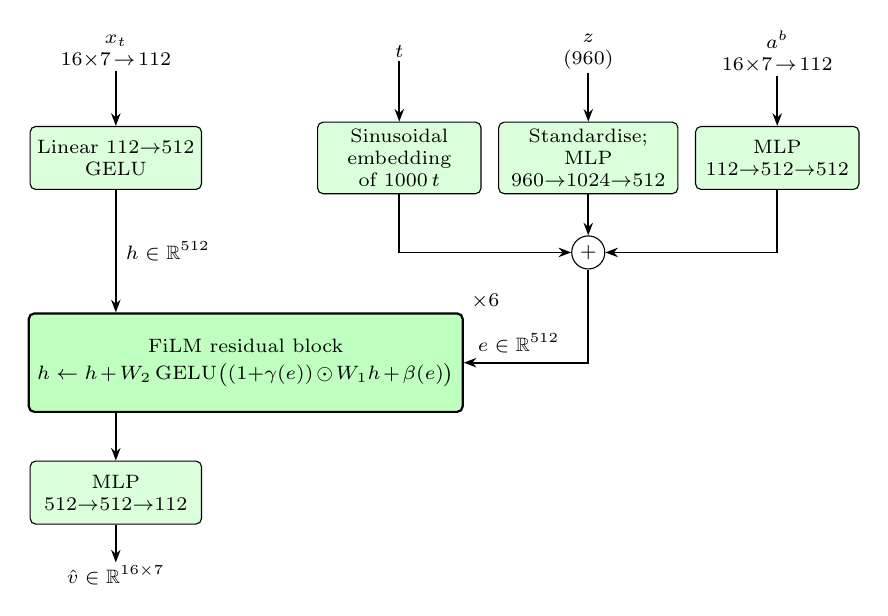
\begin{tikzpicture}[
    font=\scriptsize, >={Stealth[length=1.6mm]},
    io/.style={align=center, inner sep=1pt},
    lay/.style={draw, rounded corners=2pt, fill=green!14, align=center, inner sep=2.5pt, text width=1.55cm, minimum height=0.8cm},
    blk/.style={draw, rounded corners=2pt, fill=green!25, align=center, inner sep=3pt, text width=3.0cm, minimum height=1.25cm, thick},
    arr/.style={->, semithick}
]
\node[io] (xt) at (0,0) {$x_t$\\$16{\times}7\!\to\!112$};
\node[io] (t)  at (3.6,0) {$t$};
\node[io] (z)  at (6.0,0) {$z$\\(960)};
\node[io] (ab) at (8.4,0) {$a^{b}$\\$16{\times}7\!\to\!112$};

\node[lay, text width=2.0cm] (lin) at (0,-1.35) {Linear $112{\to}512$\\GELU};
\node[lay, text width=1.9cm] (te) at (3.6,-1.35) {Sinusoidal\\embedding of $1000\,t$};
\node[lay, text width=2.1cm] (ze) at (6.0,-1.35) {Standardise; MLP\\$960{\to}1024{\to}512$};
\node[lay, text width=1.9cm] (ae) at (8.4,-1.35) {MLP\\$112{\to}512{\to}512$};
\node[draw, circle, inner sep=0.5pt, minimum size=0.42cm] (sum) at (6.0,-2.55) {$+$};

\node[blk, text width=5.3cm] (film) at (1.65,-3.95) {FiLM residual block\\[2pt]$h\leftarrow h+W_2\,\mathrm{GELU}\bigl((1{+}\gamma(e))\odot W_1h+\beta(e)\bigr)$};
\node[io, anchor=south west] at ($(film.north east)+(0.05,0.0)$) {$\times 6$};
\node[lay, text width=2.0cm] (out) at (0,-5.6) {MLP\\$512{\to}512{\to}112$};
\node[io] (v) at (0,-6.65) {$\hat v\in\mathbb{R}^{16\times 7}$};

\draw[arr] (xt) -- (lin); \draw[arr] (t) -- (te); \draw[arr] (z) -- (ze); \draw[arr] (ab) -- (ae);
\draw[arr] (te.south) |- (sum.west); \draw[arr] (ze) -- (sum); \draw[arr] (ae.south) |- (sum.east);
\draw[arr] (lin.south) -- (lin.south |- film.north) node[midway, right] {$h\in\mathbb{R}^{512}$};
\draw[arr] (sum.south) |- (film.east) node[pos=0.78, above] {$e\in\mathbb{R}^{512}$};
\draw[arr] (out.north |- film.south) -- (out.north); \draw[arr] (out) -- (v);
\end{tikzpicture}}
\caption{Architecture of the residual flow head $v_\theta$. The noisy residual chunk is flattened and projected to a 512-D hidden vector $h$. Flow time, the semantic feature and the base action chunk are embedded separately and summed into one conditioning vector $e$, which modulates each of six residual blocks through a feature-wise scale $\gamma(e)$ and shift $\beta(e)$. The output is the predicted velocity for all 16 steps of the chunk.}
\label{fig:head}
\end{figure}

Fig.~\ref{fig:head} shows the network. The noisy chunk $x_t$ is flattened to 112 values and projected to a hidden vector $h\in\mathbb{R}^{d}$ with $d=512$. The conditioning vector is the sum of three embeddings,
\begin{equation}
    e=\phi_t(1000\,t)+\phi_z(\tilde z)+\phi_a(a^{b}),
\end{equation}
where $\phi_t$ is a sinusoidal embedding and $\phi_z$, $\phi_a$ are two-layer MLPs. Flow time is multiplied by 1000 before the sinusoidal embedding because the embedding's frequencies are designed for integer diffusion steps and barely resolve $t\in[0,1]$ otherwise. The trunk is a stack of six residual blocks with FiLM conditioning~\cite{film},
\begin{equation}
    h\leftarrow h+W_2\,\mathrm{GELU}\bigl((1+\gamma(e))\odot W_1h+\beta(e)\bigr),
\end{equation}
followed by a two-layer MLP that outputs the velocity for the whole chunk. The head has 8.5\,M parameters.

\subsection{Training on a Feature Cache}
Since the backbone is frozen, everything the head needs from it is a deterministic function of the observation (the feature $z$) or can be pre-sampled (the base chunk $a^{b}$). Training therefore proceeds in two stages (Fig.~\ref{fig:architecture}b).

\textbf{Stage 1: cache.} For every frame of every demonstration of the task, the recorded simulator state is restored in the LIBERO simulator and the observation is rendered through the same code path that the evaluation uses ($256\times256$ images rotated by $180^\circ$, the same state vector and the same SmolVLA pre-processor). This removes any mismatch between the stored demonstration images and what the policy sees at rollout. The frozen SmolVLA is run once on each frame and we store $z$, $K=4$ independent samples $a^{b}_{1},\dots,a^{b}_{K}$ of the base chunk, and the normalised demonstration chunk $a^{\star}$. For task 3 this gives 12{,}434 frames from 50 demonstrations.

\textbf{Stage 2: head training.} Each optimisation step draws a mini-batch of frames, picks one of the $K$ cached base samples per frame uniformly at random, forms the residual of Eq.~\eqref{eq:residual} and minimises Eq.~\eqref{eq:loss}. Using several base samples per frame exposes the head to the variability of the base policy without re-running the backbone. As an augmentation, Gaussian noise with standard deviation 0.5 is added to the standardised feature $\tilde z$ during training, which reduces over-fitting to the small number of demonstrations. We train with AdamW (learning rate $3\times10^{-4}$ with cosine decay, weight decay $10^{-4}$, batch size 256, gradient-norm clipping at 1) for 300 epochs and keep an exponential moving average of the weights (decay 0.999), which is the model that is evaluated. Stage 1 takes about 40 minutes for one task on a single laptop GPU and Stage 2 about two minutes.

\subsection{Closed-Loop Inference}
At control step $k$ the policy executes
\begin{equation}
    u_k=\mathrm{clip}\bigl(\mathrm{unnorm}\bigl([\,a^{b}+\alpha\,\hat r\,]_{1}\bigr),-1,1\bigr),
\end{equation}
where $[\cdot]_1$ selects the first action of the chunk, $\mathrm{unnorm}$ maps back to environment units and $\alpha$ scales the correction ($\alpha=1$ in our experiments; $\alpha=0$ recovers the base policy). The base chunk and the residual are produced from the same observation and the same prefix pass, and the residual is conditioned on exactly the base chunk it is added to. A new chunk is generated at every control step, which is also how the base SmolVLA checkpoint is run (it executes one action per predicted chunk). Clipping is applied in environment units, after un-normalisation, because $\pm1$ in the normalised space corresponds to only one standard deviation of the action distribution.

\section{Experiments}

\subsection{Setup}
We evaluate on LIBERO-10~\cite{libero}. Each task provides 50 demonstrations and 50 benchmark initial states. An episode starts from a benchmark initial state, runs 10 no-op steps to let the scene settle, and then executes the policy with operational-space delta-pose control for at most 520 steps; it counts as a success if the task's goal predicate becomes true. The frozen base policy and the residual policy are evaluated through the same code path on the same initial states, with the random seed of the sampling noise set from the episode index, so the comparison is paired. We report the number of successes, Wilson 95\% confidence intervals and an exact McNemar test on the paired outcomes.

Head width, depth and the feature-noise level were selected on five held-out demonstrations of task 3 using the action error defined below, not on rollouts. The head evaluated in simulation was trained on the remaining 45 demonstrations.

\subsection{Offline Action Error}
Before running rollouts we measure, on held-out demonstration frames, how close the first action of the chunk is to the demonstrated action with and without the correction (Table~\ref{tab:offline}). The residual reduces the first-step squared error by about 25\% on unseen demonstrations. The gap between training and held-out error is large, which reflects the small data set (45 demonstrations) rather than limited model capacity.

\begin{table}[t]
\centering
\caption{Offline action error on task 3 (mean squared error to the demonstrated action, normalised action units, lower is better).}
\label{tab:offline}
\begin{tabular}{lcc}
\toprule
 & Base $a^{b}$ & Base + residual \\
\midrule
First action, held-out demos (5) & 0.462 & 0.345 \\
Full 16-step chunk, held-out demos (5) & 0.373 & 0.362 \\
First action, training demos (45) & 0.556 & 0.037 \\
\bottomrule
\end{tabular}
\end{table}

\subsection{Closed-Loop Results}
Table~\ref{tab:results} lists closed-loop success. On task 3 (\emph{put the black bowl in the bottom drawer of the cabinet and close it}) the frozen base policy succeeds in 43 of 50 episodes (86\%, 95\% CI 74--93\%) and the residual policy in 48 of 50 (96\%, 95\% CI 87--99\%). Looking at the paired outcomes, the residual policy solves six initial states on which the base policy fails and fails on one that the base policy solves; one initial state is failed by both. With seven discordant pairs the exact McNemar test gives $p=0.125$, so at this sample size the improvement cannot be distinguished from chance. Successful episodes take a similar number of steps under both policies (256 for the base policy and 268 for the residual policy on average).

\begin{table}[t]
\centering
\caption{Closed-loop success on LIBERO-10. ``Reference'' is the frozen base policy evaluated with the standard LeRobot evaluation script (3 seeds $\times$ 10 episodes). ``Base'' and ``Residual'' are evaluated with our harness on the 50 benchmark initial states of each task (successes out of 50). Rows marked -- have not been run yet.}
\label{tab:results}
\begin{tabular}{ccccc}
\toprule
Task & Reference (\%) & Base & Residual & $p$ (McNemar) \\
\midrule
0 & 16.7 & -- & -- & -- \\
1 & 36.7 & -- & -- & -- \\
2 & 40.0 & -- & -- & -- \\
3 & 83.3 & 43/50 & 48/50 & 0.125 \\
4 & 0.0  & -- & -- & -- \\
5 & 90.0 & -- & -- & -- \\
6 & 70.0 & -- & -- & -- \\
7 & 10.0 & -- & -- & -- \\
8 & 13.3 & -- & -- & -- \\
9 & 46.7 & -- & -- & -- \\
\midrule
Mean & 40.7 & -- & -- & \\
\bottomrule
\end{tabular}
\end{table}

\subsection{Limitations of the Current Evidence}
The closed-loop result covers a single task, a single training seed for the head and 50 episodes. Task 3 is also one on which the base policy is already strong, which leaves little room for improvement; tasks on which the base policy succeeds less often are more informative and are being evaluated. All 50 benchmark initial states of the task are used, so stronger evidence has to come from additional tasks and training seeds rather than from more episodes on this task. Finally, the head is trained per task.

\section{Conclusion}

[To be completed once the LIBERO-10 evaluation in Table~\ref{tab:results} is finished. The conclusion should state whether a frozen-backbone residual flow head improves the base policy across tasks, and on which kind of task it helps or hurts.]

\begin{thebibliography}{00}
\bibitem{rt2} A. Brohan \emph{et al.}, ``RT-2: Vision-language-action models transfer web knowledge to robotic control,'' in \emph{Proc. Conf. Robot Learning (CoRL)}, 2023.
\bibitem{openvla} M. J. Kim \emph{et al.}, ``OpenVLA: An open-source vision-language-action model,'' in \emph{Proc. Conf. Robot Learning (CoRL)}, 2024.
\bibitem{pi0} K. Black \emph{et al.}, ``$\pi_0$: A vision-language-action flow model for general robot control,'' arXiv:2410.24164, 2024.
\bibitem{smolvla} M. Shukor \emph{et al.}, ``SmolVLA: A vision-language-action model for affordable and efficient robotics,'' arXiv:2506.01844, 2025.
\bibitem{libero} B. Liu \emph{et al.}, ``LIBERO: Benchmarking knowledge transfer for lifelong robot learning,'' in \emph{Advances in Neural Information Processing Systems (NeurIPS)}, 2023.
\bibitem{diffusionpolicy} C. Chi \emph{et al.}, ``Diffusion policy: Visuomotor policy learning via action diffusion,'' in \emph{Proc. Robotics: Science and Systems (RSS)}, 2023.
\bibitem{ddpm} J. Ho, A. Jain, and P. Abbeel, ``Denoising diffusion probabilistic models,'' in \emph{Advances in Neural Information Processing Systems (NeurIPS)}, 2020.
\bibitem{flowmatching} Y. Lipman, R. T. Q. Chen, H. Ben-Hamu, M. Nickel, and M. Le, ``Flow matching for generative modeling,'' in \emph{Proc. Int. Conf. Learning Representations (ICLR)}, 2023.
\bibitem{residualpolicy} T. Silver, K. Allen, J. Tenenbaum, and L. Kaelbling, ``Residual policy learning,'' arXiv:1812.06298, 2018.
\bibitem{residualrl} T. Johannink \emph{et al.}, ``Residual reinforcement learning for robot control,'' in \emph{Proc. IEEE Int. Conf. Robotics and Automation (ICRA)}, 2019.
\bibitem{film} E. Perez, F. Strub, H. de Vries, V. Dumoulin, and A. Courville, ``FiLM: Visual reasoning with a general conditioning layer,'' in \emph{Proc. AAAI Conf. Artificial Intelligence}, 2018.
\end{thebibliography}

\end{document}
